\section{Methods}

In order to demonstrate that the DISHTINY platform selects for detectable hierarchical transitions in individuality, we performed experiments where cells controlled by evolving genetic programs evolved open-ended behaviors to make decisions about resource sharing, reproductive timing, and apoptosis.
We will first cover the design of the DISHTINY platform and then describe the cell-like organisms we used to evaluate the platform.

\subsection{Resource Collection}

DISHTINY allows cell-like organisms to replicate across a toroidal grid.
Over discrete time steps (``updates''), the cells can collect a continuous-valued resource.
Once sufficient resource has been accrued, cells may pay $1.0$ resource to place a daughter cell on an adjoining tile of the toroidal grid (i.e., reproduce), replacing any existing cell already there.
Collected resource decays at a rate of 0.1\% per update, incentivizing its quick use.
As cells reproduce, they can choose to include offspring in the parent's cooperating ``signaling channel'' group or expel offspring to found a new cooperating ``signaling channel'' group.

Resource appears at a single point then spreads outwards update-by-update in a diamond-shaped wave. The expanding wave halts at a predefined limit.
Cells must enter an ``activated'' state to harvest resource as it passes overhead.
The cell at the starting position of a resource wave is automatically activated, and will propagate the activation signal to neighboring cells on the same signaling channel.
The newly activated cells, in turn, activate their own neighbors registered to the same signaling channel.
Neighbors registered to other signaling channels do not activate.
Each cell, after sending the activation signal, enters a temporary quiescent state.
In this manner, cells sharing a signaling channel track and harvest an expanding resource wave.
The rate of resource collection for a cell is determined by the size and shape of of its same-channel signaling network;
small or fragmented same-channel signaling networks will frequently miss out on resource as it passes by.

Resource waves have a limited extent.
Cells that activate outside the extent of a resource wave collect no resource.
A long quiescent period ensures that erroneously activated cells miss several subsequent opportunities to collect resource and therefore will tend to collect resource at a slower rate.
In this manner, ``Goldilocks'' --- not to small and not too big --- signaling networks enjoy superior fitness.

Resource wave starting points (seeds) are tiled over the toroidal grid from a randomly chosen starting location such that the extents of the resource waves do not overlap.
All resource waves begin and proceed synchronously;
when they complete, the next resource waves are seeded.
This process provides efficient and spatially-uniform selection for ``Goldilocks'' same-channel signaling networks.

Cells control the size and shape of their same-channel signaling group through strategic reproduction.
Three choices are afforded: whether to reproduce at all, where among the four adjoining tiles of the toroidal grid to place their offspring, and whether the offspring should be registered to the parent's signaling channel or be given a random channel ID (in the range 1 to $2^{64} - 1$).
The probability of channel collision is miniscule: $60 \times 60 \times 2^{20}$ (the grid dimensions times the number of simulation updates) independent channel values will collide with probability less than $1 \times 10^{-9}$.
No guarantees are made about the uniqueness of a newly-generated channel ID, but chance collisions are rare.

Hierarchical levels are introduced into the system through multiple separate, but overlaid, instantiations of this resource wave/channel-signaling scheme.
We refer to each independent resource wave/channel-signaling system as a ``level.''
In some experimental treatments, we allowed two resource wave/channel-signaling levels, identified here as level one and level two.
On level one, resource waves extended a radius of two toroidal tiles.
On level two they extended a radius of six toroidal tiles.
On both levels, activated cells netted $+0.2$ resource from a resource wave, but did not collect any resource outside the extent of the resource wave.
Due to the different radii of resource waves on different levels, level one selects for small same-channel signaling networks and level two selects for large same-channel signaling networks.

Each cell contained a pair of separate channel IDs, the first for level one and the second for level two.
We kept these channel IDs hierarchically nested by constraining inheritance during reproduction.
Daughter cells could not inherit just the level-one channel ID, they could either
\begin{enumerate}
\item inherit both level-one and level-two channel ID,
\item inherit level-two channel ID but not level-one channel ID, or
\item inherit neither channel ID.
\end{enumerate}
Hierarchically nested channel IDs are analogous to a strict corporate organizational structure: all employees (i.e., cells) are members of one department (i.e., level-one channel network) and one corporation (i.e., level-two channel network) but no employee can be a member of two departments and no department can be a member of two corporations.
Figure \ref{fig:morphology-wt} depicts hierarchically nested channel states assumed by an evolved strain.

An evolutionary transition in individuality can readily be evaluated within the DISHTINY framework with respect to same-channel network groups.
In addition to a potentially functionally cooperative relationship, shared channel IDs --- which may only systematically arise through inheritance --- imply a close hereditary relationship.
Because new channel IDs arise first in a single cell, same-channel signaling networks are reproductively bottlenecked analogously to a "Staying Together" life cycle (rather than a "Coming Together" life cycle) \cite{staps2019emergence}.
This precludes chimeric groups, except for mutations arising from somatic reproduction and rare cases of channel ID collision.

To recognize an evolutionary transition in individuality, we can evaluate
\begin{enumerate}
\item whether cells with the same channel ID cooperate altruistically by assessing, for example, resource sharing, and
\item whether delegation of reproductive labor arises by assessing whether interior cells cede reproduction to those at the periphery.
\end{enumerate}
If cells sharing the same level-one channel fulfill these conditions, we would suppose that a first-level transition in individuality had occurred.
Likewise, if cells sharing the sharing the same level-two channel fulfill these conditions, we would suppose that a second-level transition in individuality had occurred.
Further, we can screen for the evolution of complex multicellularity by assessing cell-cell messaging, regulatory patterning, and functional differentiation between cells within the a same-channel signaling network \cite{knoll2011multiple}.

\subsection{Channel Group Life Cycle}

Mature same-channel resource collecting groups enjoy a considerable advantage over fledging propagules.
Because of the isometric scaling relationship between surface area and perimeter, cooperative same-channel resource collecting groups can marshal more resource at their periphery.
In addition, because of their greater surface area, mature same-channel resource collecting groups are able to seed resource-wave events and collect resource at a higher per-cell rate.

In order to ensure channel group turnover and facilitate channel group propagation, we impose a timed phase-out of somatic reproduction and resource wave harvests.
For each cell, we track a channel generation counter at each resource wave level.
At the genesis of a new channel group, these counters are set to zero.
Daughter cells that expand a channel group's soma are initialized to a counter value one greater than their parent.
Additionally, all channel generation counters are incremented every 512 updates to ensure that soma ages even in the absence of reproduction.
When a cell's channel generation counter reaches 1.5 times the wave radius of its level, it can no longer produce somatic daughter cells.
Then, after two additional counter steps, cells lose their ability to seed resource wave events and collect resource.
Thus, as channel groups age over time, their constituent cells lose the ability regenerate somatic tissue and then, soon after, to collect resource.
To prevent complete stagnation in the case where all cells' channel generation counters expire we provide a uniform inflow of $+0.0051$, sufficient for one reproduction approximately every thousand updates.

Interaction between nested channel groups produces a notable selective byproduct.
Because smaller, level-one channel groups tend to have intrinsically shorter lifespans, in order to achieve the full potential productive somatic lifespan of a larger, level-two channel group its constituent small channel groups must be intermittently regenerated.
Otherwise, the soma's capacity to seed resource-wave events and to collect resource will be prematurely lost once its constituent smaller, level-one channel groups expire.

This aging scheme's design ultimately stems from a desire
\begin{enumerate}
\item to facilitate evolution through regular turnover of emergent individuals and
\item to scaffold workable propagation for primitive cellular strategies while furnishing opportunities for more sophisticated adaptations to the imposed life cycle constraints.
\end{enumerate}
However, in some sense the aging scheme is heavy-handed, in effect enforcing rather than enabling a birth-death life cycle.
The evolutionary basis of aging and mortality --- in particular, the possibility of intrinsic evolutionary adaptations promoting these phenomena in addition to extrinsic factors  --- remains an active topic of scientific discussion \cite{baig2014evolution}.
In future work, we are interested in evaluating the outcomes of relaxing constraints of this aging scheme under different evolutionary conditions (such as cosmic ray mutations or irregular population structure) in light of theory attributing mortality and aging to evolvability, mutational accumulation, and costly somatic maintenance.

\subsection{Cell-Level Organisms}

\begin{figure}
\begin{center}

\hspace*{\fill}%
\begin{minipage}[t]{\columnwidth}
\centering
\vspace{0pt} % for alignment
\begin{subfigure}[b]{\textwidth}
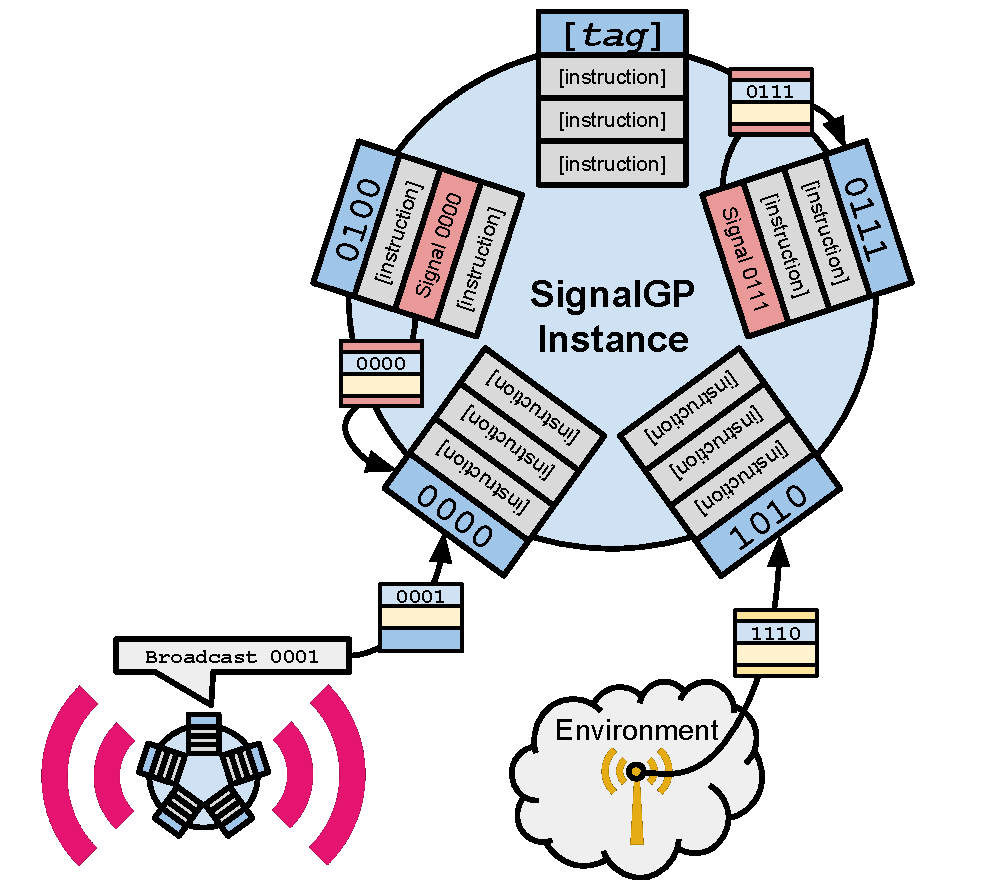
\includegraphics[width=\textwidth]{img/signalgp-cartoon}%
\caption{
A cartoon overview of a single SignalGP instance.
SignalGP program modules execute pseudo-concurrently in response to tagged signals, which can originate internally, from the environment, or from other agents.
}
\label{fig:signalgp-cartoon}
\end{subfigure}
\end{minipage}%
\hspace*{\fill}

\hspace*{\fill}%
\begin{minipage}[t]{\columnwidth}
\centering
\vspace{0pt} % for alignment
\begin{subfigure}[b]{\textwidth}
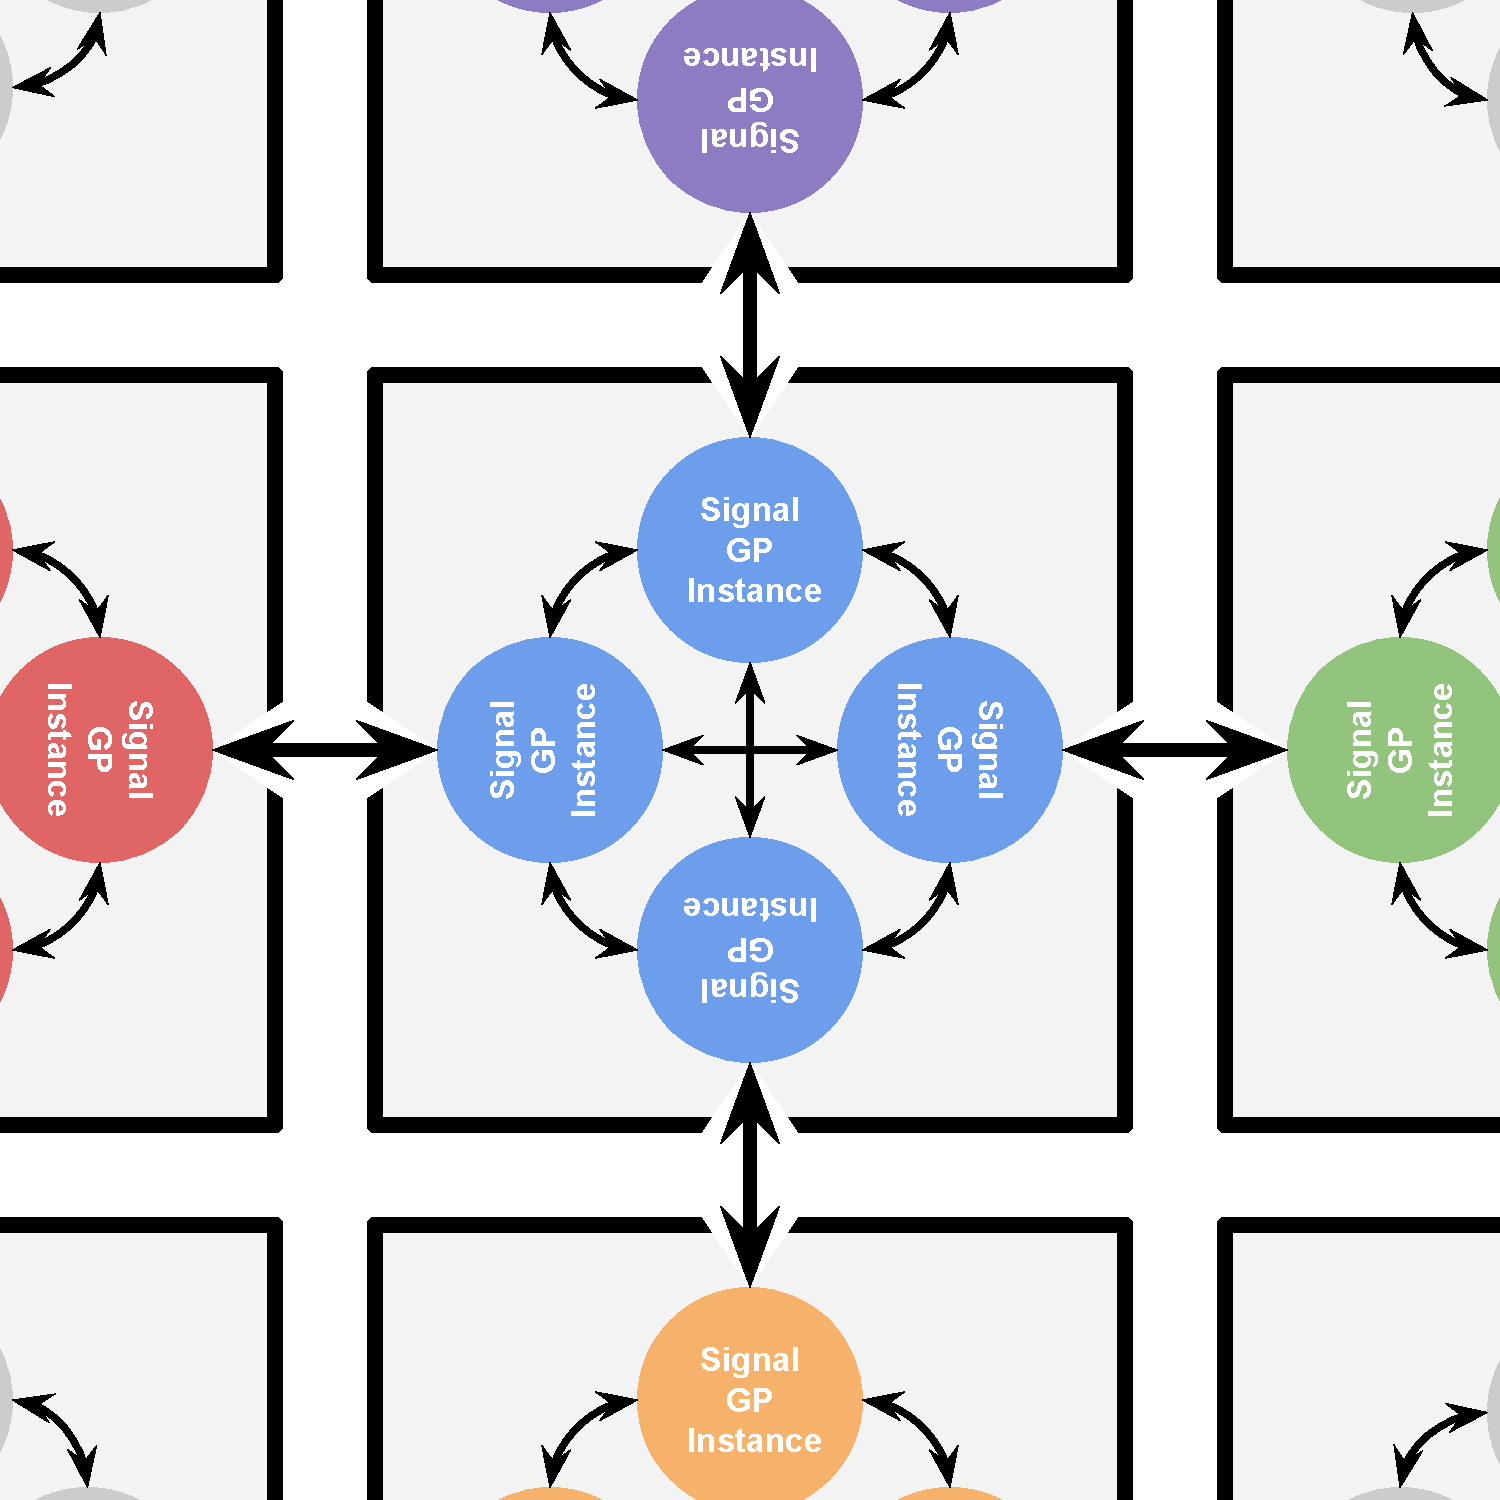
\includegraphics[width=\textwidth]{img/dishtinygp-cartoon}
\caption{
A cartoon overview of how individual SignalGP instances are organized into DISHTINY cells.
% Each cell contains four independent SignalGP instances.
% The same genetic program is mirrored across all four SignalGP instances, but each instance executes independently.
Within each DISHTINY cell, each of four independent instances senses environmental state, receives intercellular messages, and determines cell behavior with respect to a single cardinal direction.
All four instances sense non-directional environmental cues and non-directional actions may be taken by any instance.
Instances within a cell communicate via intracellular messaging.
}
\label{fig:dishtinygp-cartoon}
\end{subfigure}
\end{minipage}%
\hspace*{\fill}


\caption{
Schematic illustrations of how individual SignalGP instances function and how individual SignalGP instances are organized into DISHTINY cells.
Figure \ref{fig:signalgp-cartoon} provided courtesy Alexander Lalejini.
}
\label{fig:signalgp-dishtinygp}
\end{center}
\end{figure}


We performed our experiments using cell-level digital organisms controlled by evolving SignalGP programs.
SignalGP is genetic programming framework designed around the event-driven programming paradigm \cite{lalejini2018evolving}.
SignalGP programs are collections of independent procedural functions, each equipped with a bit-string tag.
A function is triggered by a signal with affinity that maximally and sufficiently matches its tag.
(A binding threshold of 0.1 was used in these experiments).
Signals may be generated by the environment, received as messages from other agents, or triggered internally by function execution.
Signals, and the ensuing chains of procedural execution they give rise to, are processed pseudo-concurrently by 24 virtual CPU cores.
Figure \ref{fig:signalgp-cartoon} schematically depicts a single SignalGP instance.

In this work, we introduce a regulatory extension to the SignalGP system.
During runtime, instructions may increase or decrease each tagged function's intrinsic tendency to match with --- and activate in response to --- tagged queries.
Intrinsic tag-to-tag match distances $m$ are modulated by a regulator value $r$ (baseline, 1.0) to become $r + r \times m$.
This scheme allows a function to be upregulated such that every query activates that function (e.g., $r = 0$) or no query activates that function (e.g., $r = \texttt{inf}$).
These regulation settings are heritable during reproduction but automatically decay after a number of updates determined when they are set.

To allow cells to protect themselves form potentially antagonistic interactions with their neighbors, we filter intercellular messages through a tag-matching membrane.
At runtime, cells can embed tags in this membrane that either admit or repel incoming messages.
Messages that do not match with a membrane tag are repelled.
A message, for example, that would activate a SignalGP function containing an apoptosis instruction could be rejected while other messages are accepted.
Tags embedded in this membrane automatically decay and may also be regulated.
We also filter messages between hardware instances within the same cell through a tag-matching membrane, but the default behavior for messages with unmatched tags is admission rather than rejection.

Previous work evolving digital organisms in grid-based problem domains has relied on a single computational instance which designates a direction to act in via an explicit cardinal ``facing'' state or output \cite{goldsby2014evolutionary, goldsby2018serendipitous, grabowski2010early, biswas2014causes, lalejini2018evolving}.
Under this paradigm, a large portion of genotype space encodes behaviors that are intrinsically asymmetrical with respect to absolute or relative (depending on implementation) cardinal direction.
However, in grid-based tasks, directional phenotypic symmetry is generally advantageous.
That is --- in the absence of a polarizing external stimulus --- successful agents generally behave uniformly with respect to each cardinal direction of the grid.
In this work, each cell employs four instances of SignalGP hardware: one ``facing'' each cardinal direction.
These computational instances all execute the same SignalGP program but are otherwise decoupled and may follow independent chains of execution and develop independent regulatory states.
These instances execute round robin step-by-step in an order that is randomly drawn at the outset of each update.

Genetic encodings that exploit problem-domain symmetries are known to promote evolvability and --- ultimately --- evolved solution quality \cite{clune2011performance, cheney2014unshackling}.
We submit that this directional hardware replication protocol likely increases the fraction of genotype space that encodes cardinally-symmetric phenotypes and therefore better facilitates the evolution of high-fitness phenotypes.
In further work, we look forward to exploring the evolvability and solution quality implications of this new approach.

The single SignalGP program that is mirrored across the cell's computational instances represents the cell's genome.
Mutation, with standard SignalGP mutation parameters as in \cite{lalejini2018evolving}, is applied to 1\% of daughter cells at birth.
In addition, genomes encode the bitstrings associated with environmental events.
These bitstrings evolve at a per-bit mutation rate equivalent to the bitstring labels of SignalGP functions.

Instances within a cell may send intracellular messages to one another or intercellular messages to a neighboring cell.
Intercellular messages are received by the SignalGP instance that faces the sending cell.
Figure \ref{fig:dishtinygp-cartoon} schematically depicts the configuration of the four SignalGP instances that constitute a single DISHTINY cell as well as the instances of neighboring cells that receive extracellular messages from the focal cell.

We performed our experiments on a traditional 60-by-60 toroidal grid, supporting a population of at most 3600 individual cells.
As each cell contained four SignalGP instances, our simulations encompassed up to 14,400 virtual CPUs with up to 345,600 virtual cores.
In order to reduce the computational burden of our experiment, we intermittently advanced the virtual CPUs.
Every four updates, virtual CPUs were advanced 16 cycles.
Intracellular messages were delivered immediately after they were generated.
Intercellular messages, cached in first-in first-out inboxes with maximum capacity 16, were retrieved every four updates.
Event-driven environmental cues and Accrued cell actions were dispatched every eight updates.

Evolving programs employed combinations of the event-driven environmental cues, procedural instruction-based sensors, and procedural instruction-based actuators detailed in the following two subsections.

\subsection{Instruction Library}

In addition to the generic arithmetic, logic, utility, and program flow instructions in the default SignalGP instruction set, which is laid out in \cite{lalejini2018evolving}, we define a number of custom instructions to allow evolving programs to sense and interact with their environments, including
\begin{itemize}
\item reproduction,
\item resource sharing,
\item channel ID sensing,
\item apoptosis,
\item intracellular messaging, and
\item intercellular messaging.
\end{itemize}
We provide an listing of our experiment's instruction library in the supplementary material.

Instructions that involve an extracellular neighbor default to the cell that the executing SignalGP instance is facing.
To ensure a founding crop of viable individuals, apoptosis and program flow instructions in the initial randomly-generated population were replaced with no-op instructions.
However, these instructions were allowed to mutate in to genomes freely once evolutionary runs began.

\subsection{Event Library}

Event-driven sensing has been shown to enable evolution of SignalGP programs that more successfully react to  environmental state \cite{lalejini2018evolving}, so we supplement our instruction-based sensors with event-based input.
On a regular basis, a subset of environmental events are triggered on each SignalGP hardware based on current local environmental conditions.
The activating affinity of each event is genetically-encoded as part of the program currently executing on the hardware.
We provide a listing of our experiment's event library in the supplementary material.

\subsection{Treatments}

In this work, we screened replicates conducted under combinations of two experimental conditions:
\begin{enumerate}
\item flat versus nested hierarchical resource wave/channel-signaling levels and
\item cooperative versus independent resource collection.
\end{enumerate}

The first experimental manipulation explores the effects of hierarchical nesting of kin-sensing and/or functional cooperation.
The second manipulation explores the effects of functional cooperation.

To enact the first manipulation, we compared the nested hierarchical resource wave/channel-signaling scheme described above with a single-level scheme with waves extending six toroidal tiles.
We also increased the resource wave reward to $+0.6$ to approximately match the observed resource inflow rate of the nested scheme.
To enact the second manipulation, we removed the resource wave reward and increased the uniform resource inflow rate to $+0.0175$ in order to approximately match the net inflow rate under the dual-level wave-based scheme.
Table \ref{tab:productivity} reports productivity observed under these different conditions.

We mix and match these experimental manipulations in three treatments:
\begin{enumerate}
\item one level with even resource (``Flat-Even''),
\item one level with wave-based resource (``Flat-Wave''),
\item two levels with even resource (``Nested-Even''), and
\item two levels with wave-based resource (``Nested-Wave'').
\end{enumerate}

We ran 40 replicates under each treatment condition.
Replicates were seeded with randomly generated SignalGP programs.
To conserve disk space, we divided evolutionary runs into 262144 ($2^{18}$) update epochs and collected data in 8096 ($2^{13}$) update snapshots between epochs.
All replicates ran at least one full epoch, and all comparisons between or within treatments are conducted at this time point.
However, most replicates (156/160) were able to run to four epochs during available compute time.
We screened for and conducted case studies at the latest available data for each replicate.
All reported case studies happen to be drawn from runs that completed 4 epochs of evolution.
Table \ref{tab:systematics} reports the systematics outcomes observed under each treatment at epoch 1 and at epoch 4.

\subsection{Competition Experiments and Phenotype Assays}

We performed further experiments to develop case studies of evolved strains we manually screened from our evolutionary runs.
In these experiments, the most-abundant genotype was harvested from the end-state of evolutionary runs as the wild type strain.
We collected epigenetic state (i.e., regulatory settings) along with genetic state (i.e., SignalGP program and environmental-cue-to-tag mapping).
All further work with harvested strains was conducted under environmental conditions identical to that of the treatment they evolved in.

To analyze the relative fitness of knockout strains versus wild type, we seeded 20 $60 \times 60$ toroidal grids with ten cells of each strain, including epigenetic regulator state.
We ran competition experiments for the duration of one snapshot.
Seeded cells generally proliferated to completely fill the toroidal grid in the first quarter of the snapshot.
Competition experiment outcomes were determined by strains' relative cell populations within the grid at the end of the snapshot.

To perform phenotypic comparisons between knockout strains and wild type, we seeded ten cells of each strain onto separate $60 \times 60$ toroidal grids and then cultured them for the duration of one snapshot.

\subsection{Implementation}

We implemented our experimental system using the Empirical library for scientific software development in C++, available at \url{https://github.com/devosoft/Empirical}.
The code used to perform and analyze our experiments, our figures, data from our experiments, and a live in-browser demo of our system is available via the Open Science Framework at \url{https://osf.io/g58xk/}.
Most replicates finished within a day, but some took up to a week to complete.
